\maketitle

\section{任务分析}

在并发程序设计中,进程间的同步与协调是一个关键性问题,特别是在多进程或多线程共享资源的场景下,若没有合适的同步机制,系统将面临数据不一致、竞争条件、死锁等问题。

\subsection{进程同步}

\textbf{进程同步}是指在多个进程(或线程)并发执行时,确保它们能够按预定的方式协调执行,从而避免竞争条件、死锁等问题。通常在并发程序中,多个进程需要访问共享资源,因此必须控制对这些资源的访问,确保不同进程之间的行为不会相互干扰。

同步的目的包括:\begin{itemize}
    \item 避免竞争条件:当多个进程同时访问和修改共享资源时,可能会出现不一致的情况。进程同步确保只有一个进程能够在特定时间访问共享资源。
    \item 保证顺序执行:在某些情况下,进程的执行顺序必须是有序的,以满足某些逻辑或业务规则。
    \item 避免死锁与饥饿:确保系统资源不会导致进程无限期地等待。
\end{itemize}

同步机制通常通过以下方式实现:\begin{itemize}
    \item 互斥锁(Mutex):确保同一时刻只有一个进程能够访问共享资源。
    \item 信号量(Semaphore):控制多个进程对共享资源的访问,可以用于计数或者限制并发访问的数量。
    \item 条件变量(Condition Variables):当进程需要等待某些条件满足时,能够进行有效的等待和通知。
\end{itemize}

\subsection{读者写者问题}

\textbf{读者写者问题}是一类经典的同步问题,描述了在并发访问共享数据时,读者(读操作)和写者(写操作)之间的冲突问题。问题的核心在于如何协调多个进程在访问共享资源时,确保读取和写入操作之间不会产生冲突。

\begin{itemize}
    \item 读者可以同时访问共享资源(多个读者之间不存在冲突);
    \item 写者在写入时必须独占资源,禁止任何其他读者或写者访问;
    \item 需要在保证多个读者能够并发读取的同时,又能保证写者在写入时能够独占资源。
\end{itemize}

\subsection{读者优先与写者优先}

\textbf{读者优先}和\textbf{写者优先}是读者写者问题的两种调度策略,它们决定了如何处理多个读者和写者的请求。

在读者优先策略下,如果有多个读者和一个写者请求资源,系统优先满足读者的请求,即使有写者请求,若当前没有其他写者,读者仍然可以继续读取。这种策略提高了读操作的并发性。如果读操作远多于写操作,读者优先策略能有效提升系统吞吐量。适用于读多写少的场景,避免写操作的频繁阻塞。但是可能导致写者饥饿。因为读者在某些情况下可以无限制地访问共享资源,导致写者的请求长期无法得到满足。

写者优先策略下,系统尽可能优先满足写者的请求。即使有读者正在访问共享资源,一旦写者请求到来,读者也必须等待写者完成写操作。从而避免了写者的饥饿问题,保证写操作能够及时执行。	在写操作较为重要或频繁的场景下,能够保证系统的一致性和正确性。类似的,缺点是可能导致读者的饥饿问题。如果写者频繁获得资源,读者可能长时间无法读取数据。

\section{实验环境}

\begin{itemize}
    \item 操作系统:macOS Sequoia \texttt{15.2 (24C101)}
    \item 编程语言:c++23
    \item 编译器:clang \texttt{19.1.6}
    \item 构建工具:xmake \texttt{v2.9.7+20241219}
    \item 文档构建工具:doxygen \texttt{1.12.0}
\end{itemize}

\section{设计思路}

\subsection{读者优先}

该策略要求多个读者可以并发访问共享资源,而写者在读者完成所有读取操作之前无法进行写入操作。我们通过使用互斥锁和计数器等工具来实现这种同步机制,保证了多个读者和写者之间的有序执行。

\subsubsection{资源访问控制的分离}

为了正确实现读者优先策略,我们将资源访问控制分为两个互斥锁:\begin{itemize}
    \item 读者计数控制(\texttt{mtx}):用来追踪当前正在读取的读者数量。通过读者计数来决定是否需要阻塞写者。
    \item 写者互斥锁(\texttt{wrt}):用来确保写者在执行写操作时能够独占资源,并阻止任何其他读者或写者同时访问共享资源。
\end{itemize}

这种分离机制的关键点在于,读者的数量直接决定写者的访问权限。如果有读者正在进行读取操作,第一个进入临界区的读者会锁定写者互斥锁(\texttt{wrt}),从而阻止写者进入;当最后一个读者离开时,会释放写者互斥锁,允许等待中的写者进入。

\begin{algorithm}[htbp]
    \caption{Reader线程伪代码}
    \KwIn{$reader\_id$}  % 输入读者ID
    \While{true}{
        \textbf{入口部分} \\
        \textbf{锁} $mtx$ \\
        $read\_count \gets read\_count + 1$ \\
        \If{$read\_count == 1$}{
            \textbf{锁} $wrt$  \quad // 第一个读者锁定写者
        }
        \textbf{解锁} $mtx$  \\
        
        \textbf{关键部分(读取)} \\
        输出 "[时间戳] Reader $reader\_id$ is reading" \\
        \textbf{等待} 100ms \\
        
        \textbf{退出部分} \\
        \textbf{锁} $mtx$ \\
        $read\_count \gets read\_count - 1$ \\
        \If{$read\_count == 0$}{
            \textbf{解锁} $wrt$  \quad // 最后一个读者释放写者锁
        }
        \textbf{解锁} $mtx$ \\
        
        \textbf{等待} 100ms \quad // 模拟读者之间的间隔
    }
    \end{algorithm}
    
    \begin{algorithm}[htbp]
    \caption{Writer线程伪代码}
    \KwIn{$writer\_id$}  % 输入写者ID
    \While{true}{
        \textbf{入口部分} \\
        \textbf{锁} $wrt$  \quad // 写者独占资源
        
        \textbf{关键部分(写入)} \\
        输出 "[时间戳] Writer $writer\_id$ is writing" \\
        \textbf{等待} 150ms \\
        
        \textbf{退出部分} \\
        \textbf{解锁} $wrt$ \\
        
        \textbf{等待} 150ms \quad // 模拟写者之间的间隔
    }
\end{algorithm}

对于读者:
\begin{enumerate}
    \item 读者首先通过 \texttt{mtx} 锁来更新 \texttt{read\_count}(当前正在读取的读者数量)。
    \item 如果这是第一个读者,它会锁定 \texttt{wrt},阻止写者进入。
    \item 读者完成读取后,减少 \texttt{read\_count},如果这是最后一个读者,则释放 \texttt{wrt},允许写者进行写操作。
\end{enumerate}

对于写者:
\begin{enumerate}
    \item 写者需要获取 \texttt{wrt} 锁,确保独占资源。
	\item 写者完成写入操作后释放 \texttt{wrt},允许其他读者和写者进行操作。
\end{enumerate}

\subsubsection{读者进入与退出的同步机制}

在实现读者优先策略时,读者进入和退出共享资源的同步非常重要。通过读者计数 \texttt{read\_count} 和锁 \texttt{wrt},我们可以确保:\begin{itemize}
    \item 多个读者并发:只要没有写者正在写,多个读者可以同时读取。
	\item 写者等待:写者必须等到所有读者都完成操作后,才能获得 \texttt{wrt} 锁进行写操作。
\end{itemize}

\begin{itemize}
    \item 进入部分:每当有读者进入时,先通过 \texttt{mtx} 锁定并增加 \texttt{read\_count},如果这是第一个读者,那么它会进一步锁定 \texttt{wrt},阻止写者进入资源区域。
    \item 退出部分:当一个读者退出时,减少 \texttt{read\_count},如果这是最后一个读者,它会释放 \texttt{wrt},从而允许写者进入。
\end{itemize}

\subsubsection{写者的访问控制}

写者需要独占资源,因此它在进入时必须获取 wrt 锁。在写操作完成后,写者会释放该锁。写者的进入和退出通过 wrt 互斥锁来实现,确保在任何时候只有一个写者能够访问共享资源。

\subsubsection{读者与写者的调度}

当系统有多个读者和写者时,读者会优先于写者执行。写者在所有读者结束操作后才会获得执行机会。这样就能避免由于大量读者的存在导致写者长时间被阻塞。

虽然在读者优先策略下,写者可能需要等待较长时间,但我们避免了写者因为每次读者进入都被阻塞的情况。写者会按照顺序等待。

\subsubsection{线程模拟与调度}

通过模拟多个线程(读者与写者)的并发执行来展示读者优先策略的工作原理。每个线程代表一个读者或写者,读者线程通过不断地读取共享资源并报告其状态,写者线程则通过模拟写操作来展示其被阻塞与释放的过程。

使用 \cppinline{std::this_thread::sleep_for} 来模拟读者和写者的操作时间,从而可以观察到在高并发情况下的同步与调度。每个线程在执行时,都会根据当前的计数和锁的状态,决定是否能够访问共享资源。通过控制这些线程的执行顺序,我们能够实现读者优先的同步策略。

\subsection{写者优先}

在读者优先策略中,主要的资源访问管理问题是读者和写者之间的互斥性。读者之间可以并发访问资源,但写者必须等到没有读者在访问时才能进行写操作。这个控制相对简单,因为我们只需要确保:如果有读者在读,写者必须等待。

写者优先策略需要管理更复杂的条件,在有读者访问的情况下,写者必须等待,而在有写者等待的情况下,读者需要阻塞。为了确保写者能够优先执行,系统必须保证:写者必须在没有读者的情况下获得资源,即使有读者在读取资源,写者也应该优先等待(避免出现写者饥饿的问题)。这就需要额外的控制来处理写者和读者之间的优先级关系。

\subsubsection{资源访问控制的分离}

类似于读者优先策略,我们依然使用两个互斥锁来控制对共享资源的访问,通过这些锁和条件变量,我们能够实现以下控制:\begin{itemize}
    \item 读者访问:多个读者可以并发访问资源,但必须等到没有写者在写入时才能进入。
    \item 写者访问:写者优先于读者,写者必须等到没有任何读者在读并且没有其他写者正在写时才能进入。
\end{itemize}

\subsubsection{写者优先的调度策略}

在写者优先的策略下,写者优先的核心要求是,在有写者等待的情况下,读者必须等待,直到所有写者完成写操作。\begin{itemize}
    \item 读者线程在进入临界区时,会检查是否有写者在写。如果有写者在写,读者必须等待。
	\item 写者线程在进入临界区时,首先会检查是否没有读者在读,并且没有其他写者在写。如果满足这些条件,写者可以进入并锁定资源。
\end{itemize}

使用条件变量 \texttt{cond} 来控制线程的等待与唤醒:\begin{itemize}
    \item 读者会等待条件变量,直到没有写者在写入。
	\item 写者会等待条件变量,直到没有读者在读并且没有其他写者在写入。
\end{itemize}

\subsubsection{读者与写者的同步}

为了确保写者优先,我们在关键部分使用了互斥锁来保护共享资源,并且确保写者会优先于读者执行,即使在有读者在读取时,只要写者有待处理的任务,它会在所有读者完成操作后被允许执行。只有在没有写者在写的情况下,读者才能继续读取共享资源。

\subsubsection{线程间的协调与等待}

通过使用 \cppinline{std::condition_variable} 来协调线程的调度。每当一个线程执行完自己的操作后,它会通知其他线程是否可以继续执行:\begin{itemize}
    \item 读者退出时,如果是最后一个读者退出,它会通知等待的写者可以开始写入。
	\item 写者退出时,它会通知等待的读者或其他写者继续执行。
\end{itemize}

\begin{algorithm}[htbp]
    \caption{Reader线程伪代码}
    \KwIn{$reader\_id$}  % 输入读者ID
    \While{true}{
        \textbf{锁} $mtx$ \\
        \textbf{等待条件}:等待 $write\_count == 0$  \quad // 确保没有写者在等待
        
        $read\_count \gets read\_count + 1$ \\
        \If{$read\_count == 1$}{
            \textbf{锁} $wrt$  \quad // 第一个读者锁定写者互斥锁
        }
        \textbf{解锁} $mtx$ \\
        
        \textbf{关键部分(读取)} \\
        输出 "[时间戳] Reader $reader\_id$ is reading" \\
        \textbf{等待} 100ms \\
        
        \textbf{退出部分} \\
        \textbf{锁} $mtx$ \\
        $read\_count \gets read\_count - 1$ \\
        \If{$read\_count == 0$}{
            \textbf{解锁} $wrt$  \quad // 最后一个读者释放写者互斥锁
            \textbf{通知所有线程} \quad // 唤醒等待的写者或读者
        }
        \textbf{解锁} $mtx$ \\
        
        \textbf{等待} 100ms \quad // 模拟读者之间的时间间隔
    }
    \end{algorithm}
    
    \begin{algorithm}[htbp]
    \caption{Writer线程伪代码}
    \KwIn{$writer\_id$}  % 输入写者ID
    \While{true}{
        \textbf{锁} $mtx$ \\
        $write\_count \gets write\_count + 1$ \\
        \textbf{等待条件}:等待 $read\_count == 0$ \quad // 确保没有读者在读
        \textbf{等待条件}:等待 $wrt\_locked == false$ \quad // 确保没有其他写者在写
        
        $wrt\_locked \gets true$  \quad // 标记写者锁定
        \textbf{锁} $wrt$  \quad // 锁定写者互斥锁
        
        \textbf{解锁} $mtx$ \\
        
        \textbf{关键部分(写入)} \\
        输出 "[时间戳] Writer $writer\_id$ is writing" \\
        \textbf{等待} 150ms \\
        
        \textbf{退出部分} \\
        \textbf{解锁} $wrt$ \quad // 解锁写者互斥锁
        \textbf{锁} $mtx$ \\
        $write\_count \gets write\_count - 1$ \\
        $wrt\_locked \gets false$ \\
        \textbf{通知所有线程} \quad // 唤醒等待的写者或读者
        \textbf{解锁} $mtx$ \\
        
        \textbf{等待} 150ms \quad // 模拟写者之间的时间间隔
    }
    \end{algorithm}
\begin{itemize}
    \item 读者线程:在进入临界区前,必须等待直到没有写者在进行写操作。在读者操作完毕后,若是最后一个读者,它会释放写者的互斥锁并通知其他等待线程。
	\item 写者线程:写者必须确保在没有读者在读,并且没有其他写者正在写时,才能锁定资源。写者操作结束后,会释放锁并通知所有等待的线程。
\end{itemize}

\section{系统框架及关键代码}

\subsection{获取当前时间的函数}
\begin{cppcode}
std::string current_time()
{
    auto now = std::chrono::system_clock::now();
    auto in_time_t = std::chrono::system_clock::to_time_t(now);
    auto duration = now.time_since_epoch();
    auto milliseconds = std::chrono::duration_cast<std::chrono::milliseconds>(duration) % 1000;

    std::tm buf {};
    localtime_r(&in_time_t, &buf);

    std::stringstream ss;
    ss << std::put_time(&buf, "%Y-%m-%d %X")
       << '.' << std::setw(3) << std::setfill('0') << milliseconds.count();
    return ss.str();
}
\end{cppcode}
该函数返回当前系统时间的字符串表示,包括年、月、日、时、分、秒和毫秒:
\begin{itemize}
    \item 使用 \cppinline{std::chrono::system_clock::now()} 获取当前时间点。
    \item 将时间转换为 \texttt{time\_t} 类型,并通过 \texttt{localtime\_r} 获取本地时间,没有使用传统的 \cppinline{std::localtime},确保多线程环境下的安全性。\texttt{localtime\_r} 是 POSIX 标准的线程安全函数,返回的结果存储在用户提供的 \cppinline{std::tm} 结构中。
    \item 利用 \cppinline{std::put_time} 格式化时间,并用 \cppinline{std::chrono::duration_cast} 获取毫秒部分,最后将其拼接成完整的时间字符串。
\end{itemize}

\subsection{ANSI颜色代码定义}
\begin{cppcode}
#define RESET "\033[0m"
#define GREEN "\033[32m"
#define RED "\033[31m"
\end{cppcode}
这部分代码定义了控制台输出的颜色代码。用于在终端中为输出的读者和写者信息着色:\begin{itemize}
    \item \texttt{RESET} 用于重置终端的颜色。
    \item \textcolor{green}{\texttt{GREEN}} 用于输出读者信息时使用绿色。
	\item \textcolor{red}{\texttt{RED}} 用于输出写者信息时使用红色。
\end{itemize}
从而将读者和写者的输出区分开来,方便观察。

\subsection{读者优先:\texttt{ReadersPriority} 类}

该类包含了实现读者优先策略的核心逻辑。它管理读者和写者的同步,以及记录当前有多少个读者在访问共享资源。

\subsubsection{数据成员}
\begin{cppcode}
private:
    std::mutex mtx; // 保护read_count的互斥锁
    std::mutex wrt; // 写者互斥锁
    int read_count = 0;  // 当前正在读取的读者数量
    std::mutex cout_mtx; // 保护输出的互斥锁
\end{cppcode}
\begin{itemize}
    \item \texttt{mtx}:用于保护 \texttt{read\_count} 变量,确保对读者数量的并发修改是安全的。
	\item \texttt{wrt}:用于保护写者的访问,确保同一时刻只有一个写者能够修改资源。
	\item \texttt{read\_count}:记录当前正在读取的读者数量。读者数量为零时,允许写者进行写操作。
	\item \texttt{cout\_mtx}:用于保护控制台输出的互斥锁,避免多个线程同时输出信息导致输出混乱。
\end{itemize}

\subsubsection{\texttt{reader} 方法}
\begin{cppcode}
void reader(int reader_id)
{
    while (true) {
        // 入口部分
        {
            std::unique_lock<std::mutex> lock(mtx);
            read_count++;
            if (read_count == 1) {
                wrt.lock(); // 第一个读者锁定wrt,阻止写者
            }
        }

        // 关键部分(读取)
        {
            std::lock_guard<std::mutex> lock(cout_mtx);
            std::cout << "[" << current_time() << "] "
                      << GREEN << "Reader " << reader_id << " is reading." << RESET << "\n";
        }
        std::this_thread::sleep_for(std::chrono::milliseconds(100)); // 模拟读取时间

        // 退出部分
        {
            std::unique_lock<std::mutex> lock(mtx);
            read_count--;
            if (read_count == 0) {
                wrt.unlock(); // 最后一个读者释放wrt,允许写者
            }
        }

        // 模拟读者之间的时间间隔
        std::this_thread::sleep_for(std::chrono::milliseconds(100));
    }
}
\end{cppcode}
\begin{itemize}
    \item 入口部分:当一个读者准备读取时,它会锁定 \texttt{mtx} 互斥锁并增加 \texttt{read\_count}。如果这是第一个读者,它会锁定 \texttt{wrt},阻止写者进入。
    \item 关键部分:在这部分,读者执行实际的读取操作,并输出日志,模拟读取的过程。然后使用 \texttt{std::this\_thread::sleep\_for} 模拟读取过程的延时。
    \item 退出部分:当一个读者退出时,它会减少 \texttt{read\_count}。如果这是最后一个读者,释放 \texttt{wrt} 锁,允许写者进入。
    \item 时间间隔:模拟读者之间的时间间隔,使得多次读者的访问能够间隔执行。
\end{itemize}
 
\subsubsection{\texttt{writer} 方法}
\begin{cppcode}
void writer(int writer_id)
{
    while (true) {
        // 入口部分
        wrt.lock();

        // 关键部分(写入)
        {
            std::lock_guard<std::mutex> lock(cout_mtx);
            std::cout << "[" << current_time() << "] "
                      << RED << "Writer " << writer_id << " is writing." << RESET << "\n";
        }
        std::this_thread::sleep_for(std::chrono::milliseconds(150)); // 模拟写入时间

        // 退出部分
        wrt.unlock();

        // 模拟写者之间的时间间隔
        std::this_thread::sleep_for(std::chrono::milliseconds(150));
    }
}
\end{cppcode}
\begin{itemize}
    \item 入口部分:写者首先会获取 \texttt{wrt} 锁,这样可以确保写操作是独占的,即在同一时刻只有一个写者可以执行写入。
	\item 关键部分:写者执行写入操作并输出日志,模拟写入过程的延迟。
	\item 退出部分:写操作完成后,写者释放 \texttt{wrt} 锁。
	\item 时间间隔:模拟多个写者之间的时间间隔。
\end{itemize}

\subsubsection{\texttt{main} 函数}
\begin{cppcode}
int main()
{
    ReadersPriority rw;
    std::vector<std::thread> threads;

    // 创建多个读者线程
    for (int i = 1; i <= 5; ++i) {
        threads.emplace_back(&ReadersPriority::reader, &rw, i);
    }

    // 创建多个写者线程
    for (int i = 1; i <= 2; ++i) {
        threads.emplace_back(&ReadersPriority::writer, &rw, i);
    }

    // 等待所有线程结束(在此示例中,线程将无限循环)
    for (auto& th : threads) {
        th.join();
    }

    return 0;
}
\end{cppcode}
\begin{itemize}
    \item \texttt{main} 函数创建多个读者和写者线程,并将它们存储在 \texttt{threads} 向量中。
	\item 创建 5 个读者线程,每个线程会执行 \texttt{reader} 方法,传入不同的 \texttt{reader\_id}。
	\item 创建 2 个写者线程,每个线程会执行 \texttt{writer} 方法,传入不同的 \texttt{writer\_id}。
	\item 线程等待:通过 \texttt{join} 方法等待所有线程结束。在这个例子中,由于线程内的循环是无限的,所以程序会一直运行。
\end{itemize}

\subsection{写者优先:\texttt{WritersPriority} 类}

读者可以并发读取共享资源,而写者在有任何读者的情况下必须等待,直到所有读者完成读取任务。

数据成员定义和主函数与读者优先类似,不再赘述。

\subsubsection{\texttt{reader} 方法}
\begin{cppcode}
void reader(int reader_id)
{
    while (true) {
        // 入口部分
        {
            std::unique_lock<std::mutex> lock(mtx);
            read_count++;
            if (read_count == 1) {
                wrt.lock(); // 第一个读者锁定wrt,阻止写者
            }
        }

        // 关键部分(读取)
        {
            std::lock_guard<std::mutex> lock(cout_mtx);
            std::cout << "[" << current_time() << "] "
                      << GREEN << "Reader " << reader_id << " is reading." << RESET << "\n";
        }
        std::this_thread::sleep_for(std::chrono::milliseconds(100)); // 模拟读取时间

        // 退出部分
        {
            std::unique_lock<std::mutex> lock(mtx);
            read_count--;
            if (read_count == 0) {
                wrt.unlock(); // 最后一个读者释放wrt,允许写者
            }
        }

        // 模拟读者之间的时间间隔
        std::this_thread::sleep_for(std::chrono::milliseconds(100));
    }
}
\end{cppcode}
\begin{itemize}
    \item 入口部分:每个读者线程在进入临界区前,首先使用 \texttt{mtx} 锁保护对 \texttt{read\_count} 的修改。如果当前是第一个进入的读者(\texttt{read\_count == 1}),则锁定 \texttt{wrt},阻止写者写入。
	\item 关键部分(读取):读者在此进行读取操作,并输出当前读者的状态。
	\item 退出部分:每个读者线程完成读取后,会再次使用 \texttt{mtx} 锁保护,减少 \texttt{read\_count}。如果当前是最后一个离开的读者(\texttt{read\_count == 0}),释放 \texttt{wrt} 锁,允许写者访问资源。
\end{itemize}

\subsubsection{\texttt{writer} 方法}
\begin{cppcode}
void writer(int writer_id)
{
    while (true) {
        // 入口部分
        wrt.lock();

        // 关键部分(写入)
        {
            std::lock_guard<std::mutex> lock(cout_mtx);
            std::cout << "[" << current_time() << "] "
                      << RED << "Writer " << writer_id << " is writing." << RESET << "\n";
        }
        std::this_thread::sleep_for(std::chrono::milliseconds(150)); // 模拟写入时间

        // 退出部分
        wrt.unlock();

        // 模拟写者之间的时间间隔
        std::this_thread::sleep_for(std::chrono::milliseconds(150));
    }
}
\end{cppcode}
\begin{itemize}
    \item 写者需要独占共享资源。在写者执行写入操作时,其他写者和所有读者都必须等待。
	\item 写者通过 \texttt{wrt.lock()} 直接锁定 \texttt{wrt} 来实现独占访问,保证写操作的互斥性。
\end{itemize}

\section{功能模块图与模块流程图}

由 doxygen 自动生成。

\subsection{读者优先策略}
\begin{figure}[H]
    \centering
    \begin{minipage}[t]{0.25\textwidth}
        \centering
        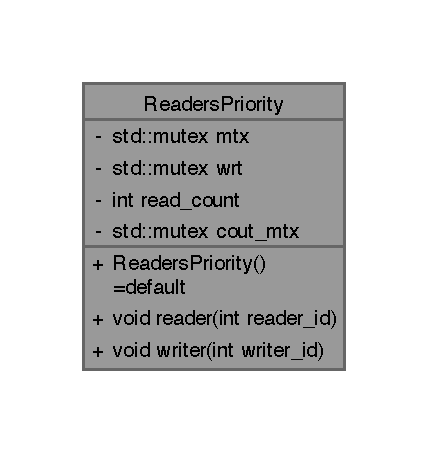
\includegraphics[width=\textwidth]{images/readerclass.pdf}
        \caption{读者优先功能模块图}
    \end{minipage}
    \begin{minipage}[t]{0.65\textwidth}
        \centering
        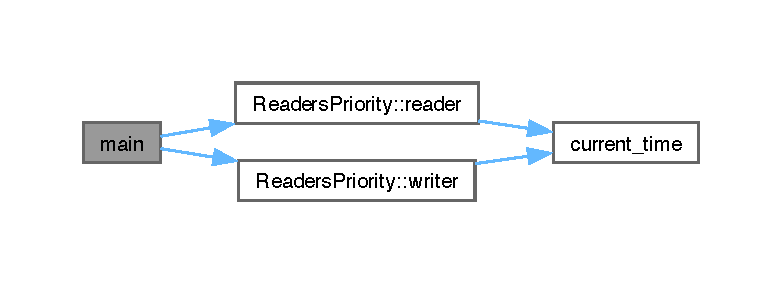
\includegraphics[width=\textwidth]{images/readerflow.pdf}
        \caption{读者优先模块流程图}
    \end{minipage}
\end{figure}

\subsection{写者优先策略}
\begin{figure}[H]
    \centering
    \begin{minipage}[t]{0.25\textwidth}
        \centering
        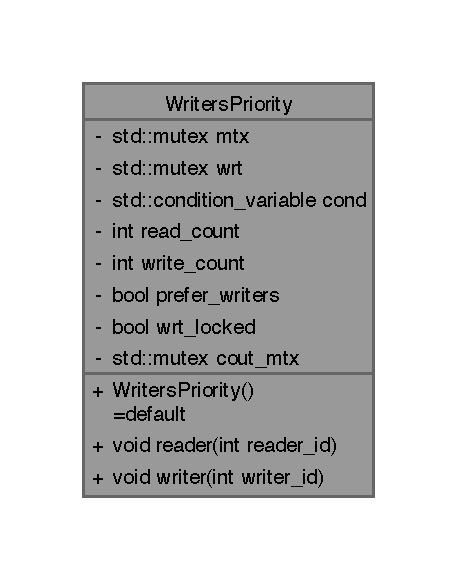
\includegraphics[width=\textwidth]{images/writerclass.pdf}
        \caption{写者优先功能模块图}
    \end{minipage}
    \begin{minipage}[t]{0.65\textwidth}
        \centering
        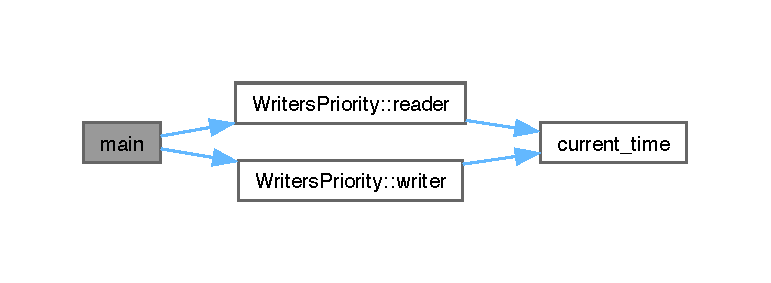
\includegraphics[width=\textwidth]{images/writerflow.pdf}
        \caption{写者优先模块流程图}
    \end{minipage}
\end{figure}

\section{测试}

稳定运行了实验报告撰写的两个小时时间。

\begin{figure}[H]
    \centering
    \begin{minipage}[t]{0.4\textwidth}
        \centering
        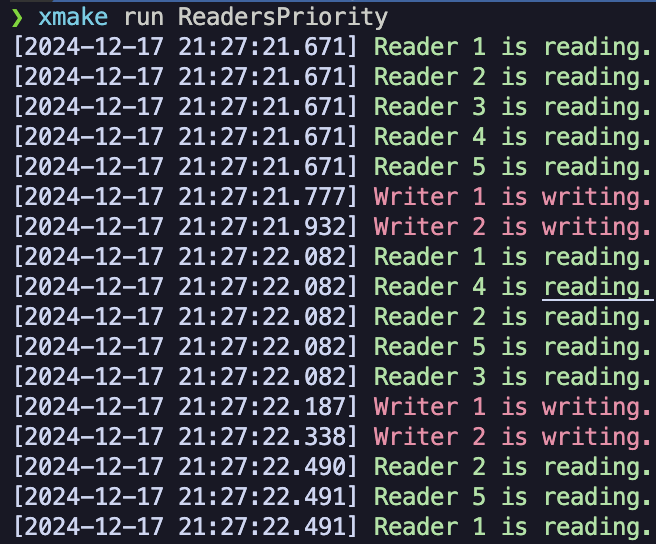
\includegraphics[width=\textwidth]{images/reader_start.png}
        \caption{读者优先运行开始}
    \end{minipage}
    \begin{minipage}[t]{0.4\textwidth}
        \centering
        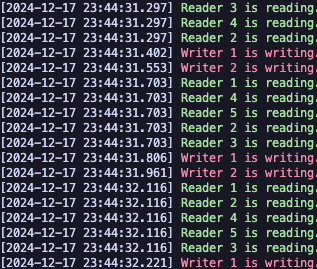
\includegraphics[width=\textwidth]{images/reader_end.png}
        \caption{读者优先运行结束}
    \end{minipage}
\end{figure}

\begin{figure}[H]
    \centering
    \begin{minipage}[t]{0.4\textwidth}
        \centering
        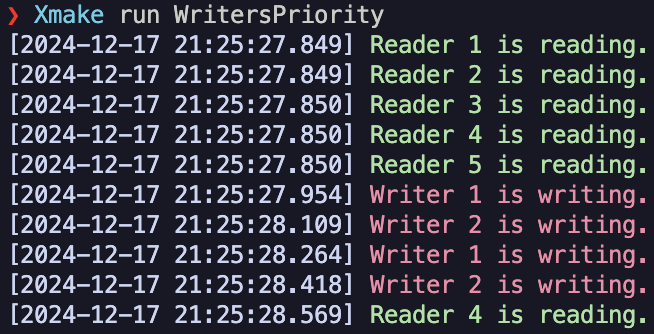
\includegraphics[width=\textwidth]{images/writer_start.png}
        \caption{写者优先运行开始}
    \end{minipage}
    \begin{minipage}[t]{0.4\textwidth}
        \centering
        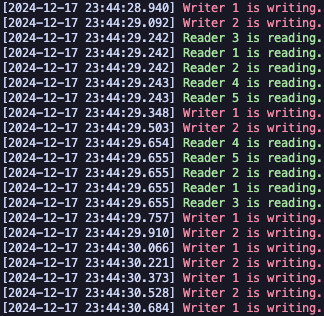
\includegraphics[width=\textwidth]{images/writer_end.png}
        \caption{写者优先运行结束}
    \end{minipage}
\end{figure}

\appendix

\section{程序文档 by doxygen}

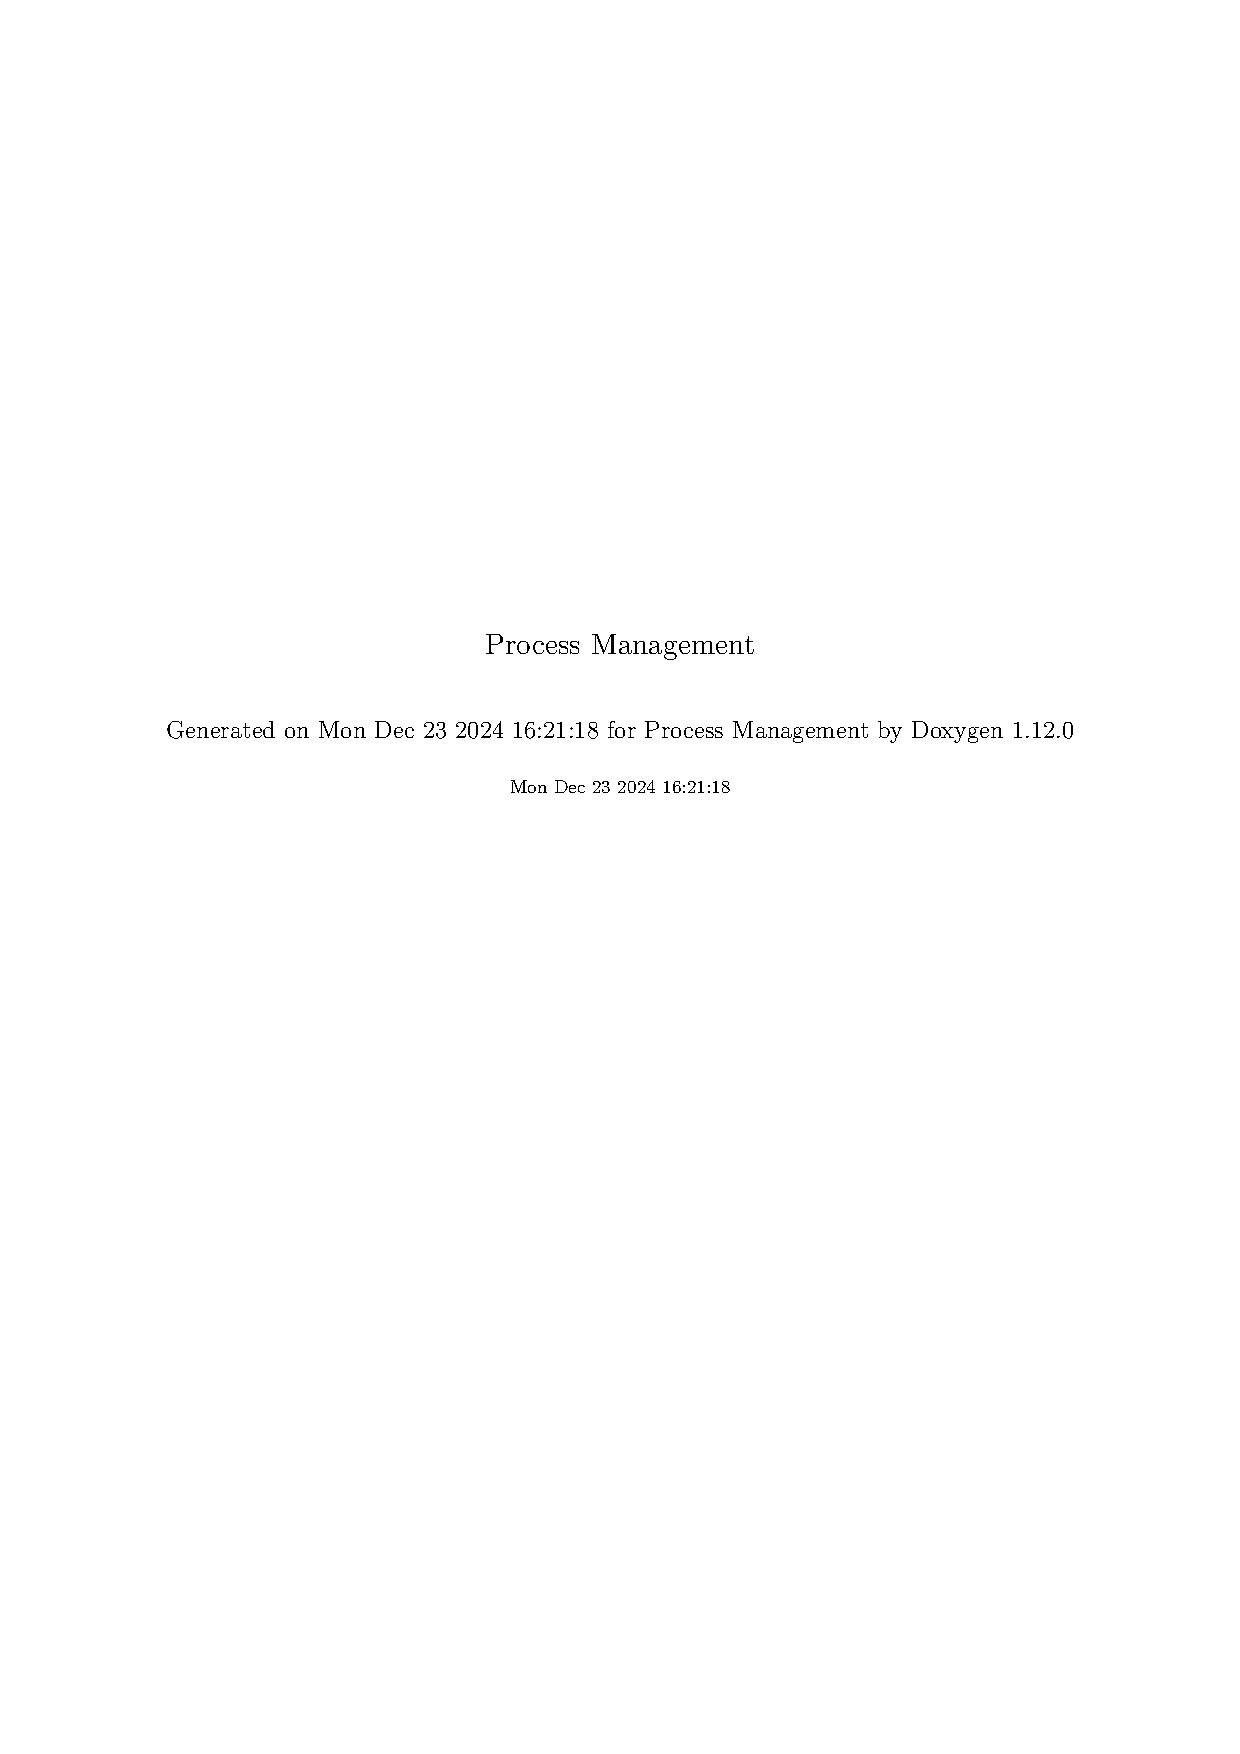
\includepdf[pages=-]{refman.pdf}